\begin{savequote}[75mm]
Often when works at a hard question, nothing good is accomplished at the first attack. Then one takes a rest, long or short, and sits down anew to the work. During the first half-hour, as before, nothing is found, and then all of a sudden the decisive idea presents itself to the mind.
\qauthor{Henri Poincare}
\end{savequote}

% pending plagiarism check
\begin{flushleft}
\chapter{Profiling of colorectal cancer organoids identifies multi-view factors of cancer organoid architecture and plasticity}


\section{Disclosure}
Large parts of this chapter have been adapted from own manuscripts, including \textit{The drug-induced phenotypic landscape of colorectal cancer organoids} \citep{Betge2022-kr}. The maximum contrast projection method, organoid segmentation method, feature extraction procedure and organoid viability classification (LDC) were previously developed by Jan Sauer as part of his dissertation \citep{noauthor_undated-ij}. Image-based profiling experiments were supported by Johannes Betge. 

\section{Image-based profiling captures the morphological diversity of patient-derived cancer organoids}

To better understand the diversity of patient derived organoid phenotypes and how their morphology was linked to biological state, I performed image-based profiling at single organoid resolution with 11 patient derived cancer organoids using compounds targeting developmental pathways (464 compounds), as well as compounds in clinical use (63 compounds in 5 concentrations, Figure \ref{fig_137} a and b genereated together with Johannes Betge). The support set contained additional gene expression profiles of untreated organoids, somatic mutation data, as well as activity information for small molecules with well-annotated targets. The resulting data comprised morphological profiles for each organoid with 528 phenotypic features  that were subsequently projected into 25 principle components, accounting for 81\% of morphological variance. 

\begin{figure}[h]
\centering
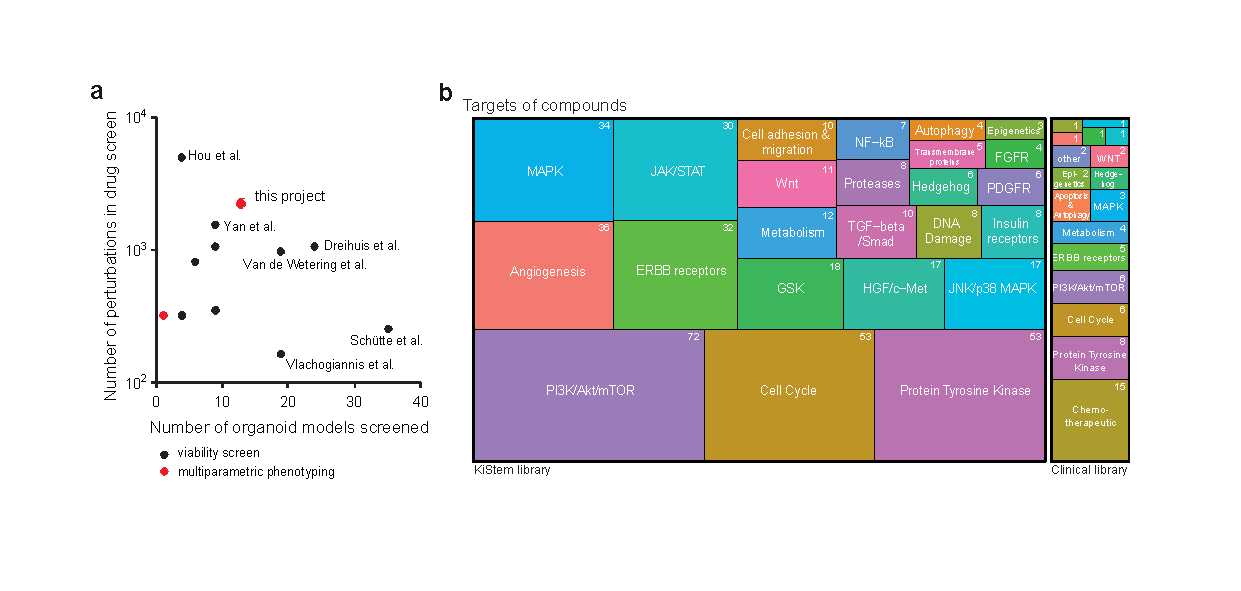
\includegraphics[width=\textwidth,
                height=\textheight,
                keepaspectratio]{figures/promise/pdf/fig_1_3.pdf}
\caption[Dataset dimensions and compound library overview]{\textbf{Dataset dimensions and compound library overview a} Number of organoid models and number of perturbations in previous publications reporting high-throughput drug screenings with patient derived cancer organoids, \textbf{b} Graphical representation of the compound libraries used for drug screening in this project: A library targeting kinases and stem cell pathways (KiStem library, 464 compounds) and a clinical library with 63 drugs in 5 concentrations. Figure created with support from Johannes Betge and adapted from \textit{The drug-induced phenotypic landscape of colorectal cancer organoids} \citep{Betge2022-kr}}
\label{fig_137}
\end{figure}

To visualize the heterogeneity of colorectal cancer organoids and drug induced changes across and within cancer organoid lines, the features of ca. 5.5 million profiled organoids were embedded using uniform manifold approximation and projection (UMAP) (Figure \ref{fig_140} a and \ref{fig_145} a-c). Most organoid lines showed characteristic bimodal log-normal distributions of organoid size with one component containing small organoids and another component made up of larger organoids with varying, line specific, average size (Figure \ref{fig_140} b, and \ref{fig_145} d-e). The log-normal-like size distribution likely resulted from intrinsic differences in cellular size and growth rate compounding over time in multicellular organoids. 

\bigbreak
While DNA and Actin staining intensity were positively correlated with organoid size, cell permeability was negatively correlated and enriched in regions with relatively smaller organoids (Figure \ref{fig_145} a-c). Graph-based clustering of this identified 12 regions within the embedding (Figure \ref{fig_140} c). When comparing drug-treated organoids to organoids treated with the negative control (DMSO), no clear separation of these two groups, except an increased presence of drug-treated organoids in region 3,  was seen. This finding suggested that organoid morphology was distributed on a continuum of phenotypes spanning perturbed and unperturbed conditions of the experiment (Figure \ref{fig_145} f). 

\clearpage

\begin{figure}[h]
\centering
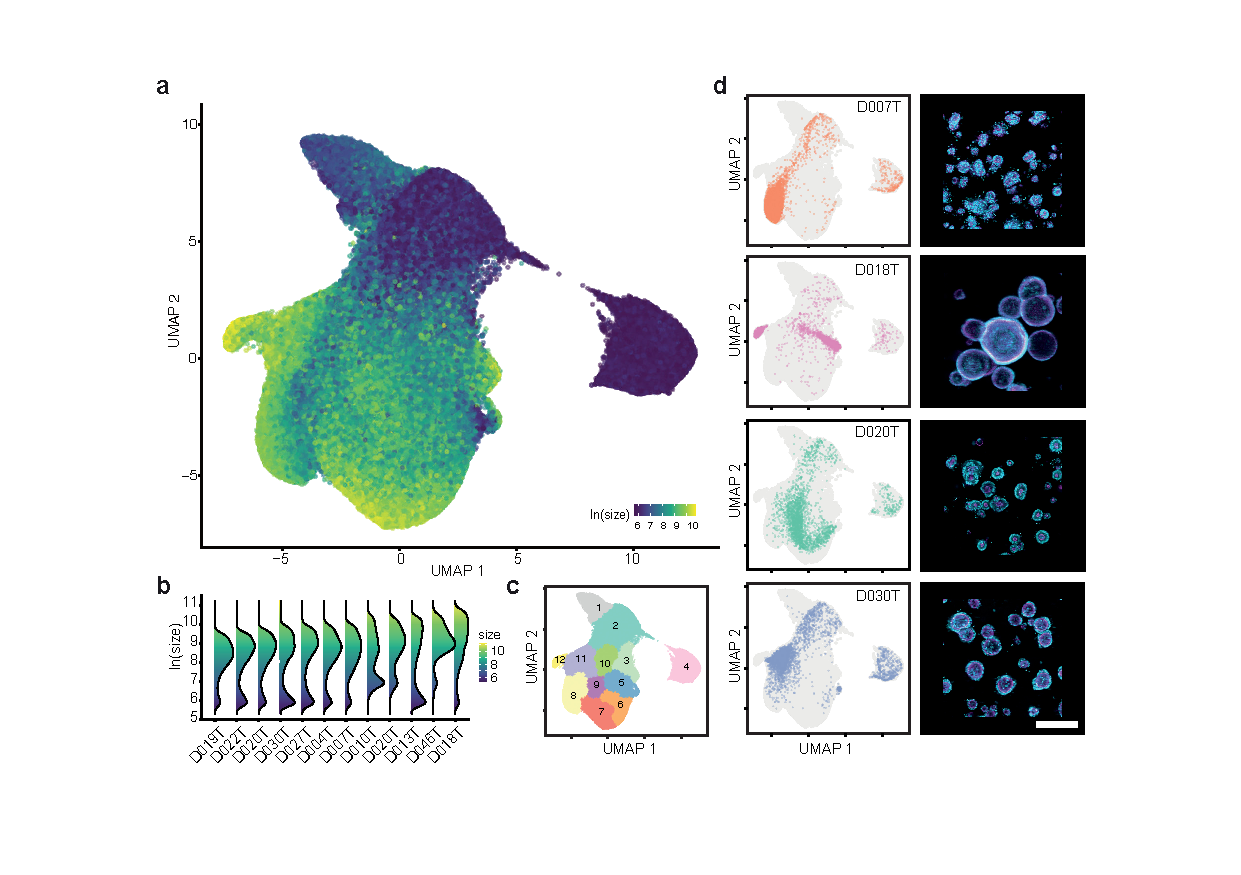
\includegraphics[width=\textwidth,
                height=\textheight,
                keepaspectratio]{figures/promise/pdf/fig_1_4.pdf}
\caption[Image-based profiling captures the phenotype diversity of patient derived cancer organoids]{\textbf{Image-based profiling captures the phenotype diversity of patient derived cancer organoids a} Uniform Manifold Approximation and Projection (UMAP) of organoid-level features for a random 5\% sample out of ca. 5.5 million organoids. The same sample is used for visualizations throughout the figure. Color corresponds to the log-scaled organoid area (dark blue: minimum size, yellow: maximum size). \textbf{b} organoid size distribution across lines. \textbf{c} UMAP representation of DMSO treated and drug treated organoids. Graph-based clustering of organoids by morphology. \textbf{d} UMAP embeddings of selected organoid lines (baseline state / 0.1\% DMSO control-treated organoids) representing different morphological subsets, grey background consists of randomly sampled points. Depicted are representative example images for each line (right, cyan = DNA, magenta = Actin, scale-bar: 200µm). Figure adapted from \textit{The drug-induced phenotypic landscape of colorectal cancer organoids} \citep{Betge2022-kr}}
\label{fig_140}
\end{figure}
\bigbreak

Different organoid lines within the embedding were located in characteristic regions, with organoid size and organoid architecture as primary organizing factors (Figure \ref{fig_140} b and d). For example, organoid line D018T had the largest median organoid size within the dataset and a cystic organoid architecture, while D020T organoids had a solid architecture and smaller median size. In most cases, organoid lines had two areas of main density, with one of them in regions 2, 3 or 4, reflecting the previously mentioned bimodal size distribution. In summary, image-based profiling of patient derived colorectal cancer organoids showed strong morphological heterogeneity with line dependent differences in size and organoid architecture.

\begin{figure}[h]
\centering
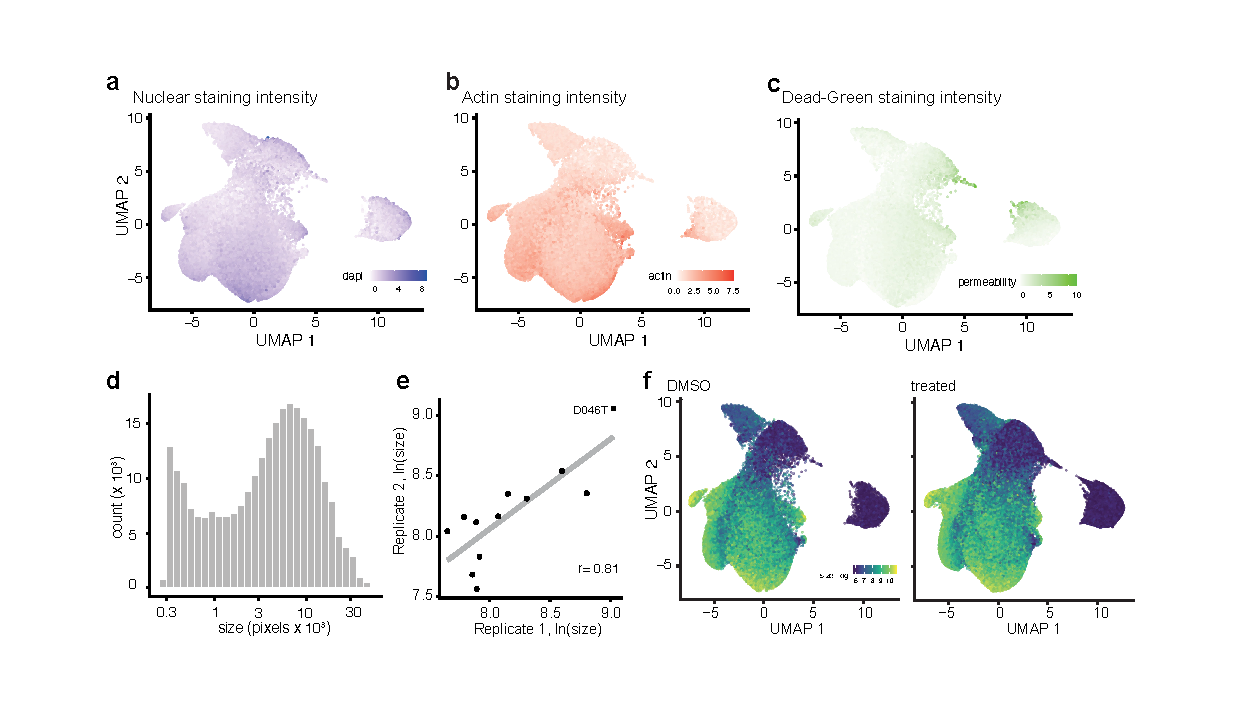
\includegraphics[width=\textwidth,
                height=\textheight,
                keepaspectratio]{figures/promise/pdf/fig_1_5.pdf}
\caption[Basic image-based features and their role in organoid phenotype diversity]{\textbf{Basic image-based features and their role in organoid phenotype diversity. a-c} Uniform Manifold Approximation and Projection (UMAP) of organoid-level features marked by DNA (DAPI) staining intensity (b), actin (Phalloidi/FITC) staining intensity (c) and permeability (DeadGreen) staining intensity \textbf{d} Distribution of organoid size for all control (DMSO) treated organoids. \textbf{e} Replicate correlation of organoid size for control treated organoids. \textbf{f} UMAP representation of DMSO treated and drug treated organoids. Figure adapted from \textit{The drug-induced phenotypic landscape of colorectal cancer organoids} \citep{Betge2022-kr}}
\label{fig_145}
\end{figure}
\bigbreak

Exploratory data analysis of the relationship between organoid morphology and experimental batch showed overall reproducible measurements of organoid profiles across experiments (Figure \ref{fig_145} e). While objects with a log-area of 8 pixels and larger showed reproducible phenotypes across contexts, smaller objects (mostly dead organoids) showed batch-dependent differences in phenotype.

\bigbreak
For example, region 1 within the UMAP embedding was exclusively occupied by observations from batch HC1092-09 and HC1092-10, while region 4 was relatively underoccupied (Figure \ref{fig_216} a). Given the confounding of line differences by experimental batches (experimental batches and tested organoid lines were not independent) and the stronger prevalence of batch effects for small objects, no procedure to remove these batch-dependent differences in organoid phenotype were performed. 

\bigbreak

\begin{figure}[h]
\centering
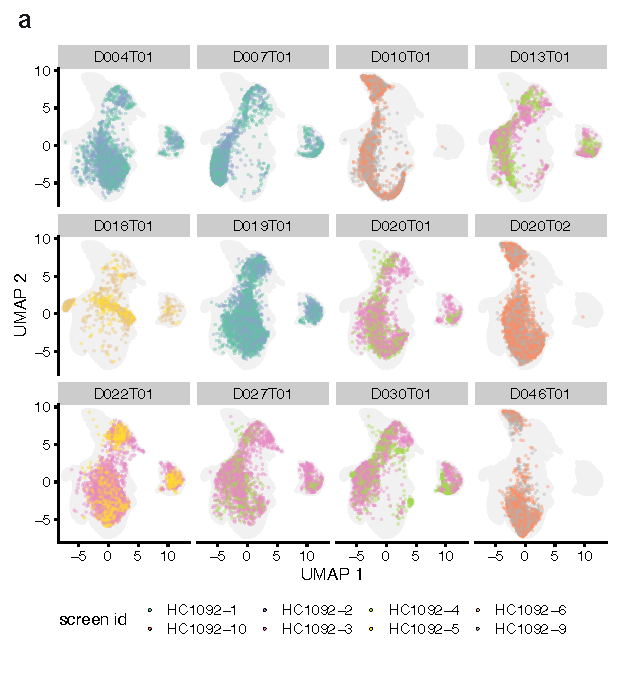
\includegraphics[width=\textwidth,
                height=\textheight,
                keepaspectratio]{figures/promise/pdf/fig_1_6.pdf}
\caption[Experimental batches and their impact on organoid phenotype]{\textbf{Experimental batches and their impact on organoid phenotype. a} UMAP of organoid level features stratified by organoid line and colored by experimental batch.}
\label{fig_216}
\end{figure}
\clearpage


\subsection{Organoid phenotype-profiles capture organoid viability}

Cell viability assays are common readouts in cancer drug discovery. Prompted by the observation that organoid size was a major factor determining the structure of the phenotype embedding (UMAP and factor 1 in MOFA analysis, see below), I hypothesized that low organoid size was at least partially the result of cell death within the organoid and, more broadly, that phenotype data could be used to estimate organoid viability. Bortezomib, a small molecule proteasome inhibitor with high in-vitro toxicity led to dose dependent organoid death in all organoid lines, thus representing suitable positive controls (Figure \ref{fig_221} a). Analogous to pseudotime in single-cell  gene expression analysis, dose-dependent trajectories of Bortezomib drug response could be fitted (Figure \ref{fig_221} b) using the non-parametric principle curve method. Starting from diverse baseline morphologies, increasing doses of Bortezomib led to a step-wise convergence on a final death-related phenotype, which corresponded to the areas with enrichment of small objects (regions 2, 3 and 4). 

\begin{figure}[h]
\centering
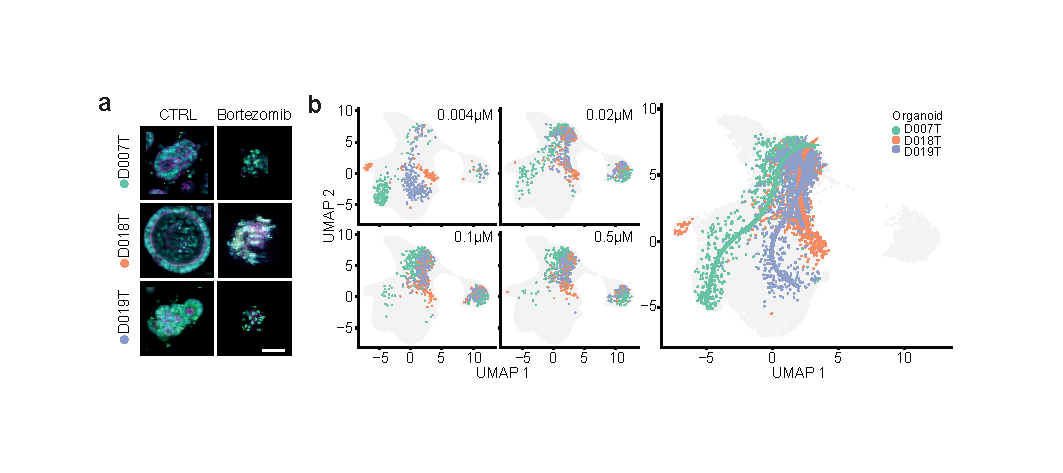
\includegraphics[width=\textwidth,
                height=\textheight,
                keepaspectratio]{figures/promise/pdf/fig_2_1.pdf}
\caption[Organoid phenotype-profiles capture organoid viability]{\textbf{Organoid phenotype-profiles capture organoid viability. a} Representative example images of negative- (0.1\% DMSO) and positive control treated organoids (2.5µM bortezomib, cyan = DNA, magenta = actin, yellow = cell permeability; average images were selected and embedded in black background; scale bar: 50µm). b, Dose-dependent-trajectory of bortezomib treatment effect. UMAP of organoid morphology at different bortezomib doses and (right panel) dose-dependent trajectory for three representative organoid lines. For visual purposes, trajectory inference was limited to partition 1, the left-hand set of measurements within the UMAP, representing ca. 95 \% of all imaging data. Panel a created with support from Johannes Betge. Figure adapted from \textit{The drug-induced phenotypic landscape of colorectal cancer organoids} \citep{Betge2022-kr}}
\label{fig_221}
\end{figure}
\bigbreak

Similarly, Paclitaxel, a microtubule disassembly inhibitor, shifted the bimodal size distribution of organoids in a dose-dependent fashion (Figure \ref{fig_222} a), while organoid count remained largely unchanged (Figure \ref{fig_222} b). This effect, however, was organoid line-specific, as median organoid size in Paclitaxel sensitive lines (e.g. D022T) decreased, while the size of other organoids remained unaffected (e.g. D046T, Figure \ref{fig_222} c-f). These observations suggested a link between organoid morphology, especially organoid size, with a loss of cell viability. 

\bigbreak
To further test the link between organoid morphology and cell viability, I performed a luminescence-based, ATP dependent, cell viability assays (CTG) in parallel with imaging as benchmark. A correlation of CTG viability with organoid size (r = 0.64) (Figure \ref{fig_222} a) was visible. 

\begin{figure}[H]
\centering
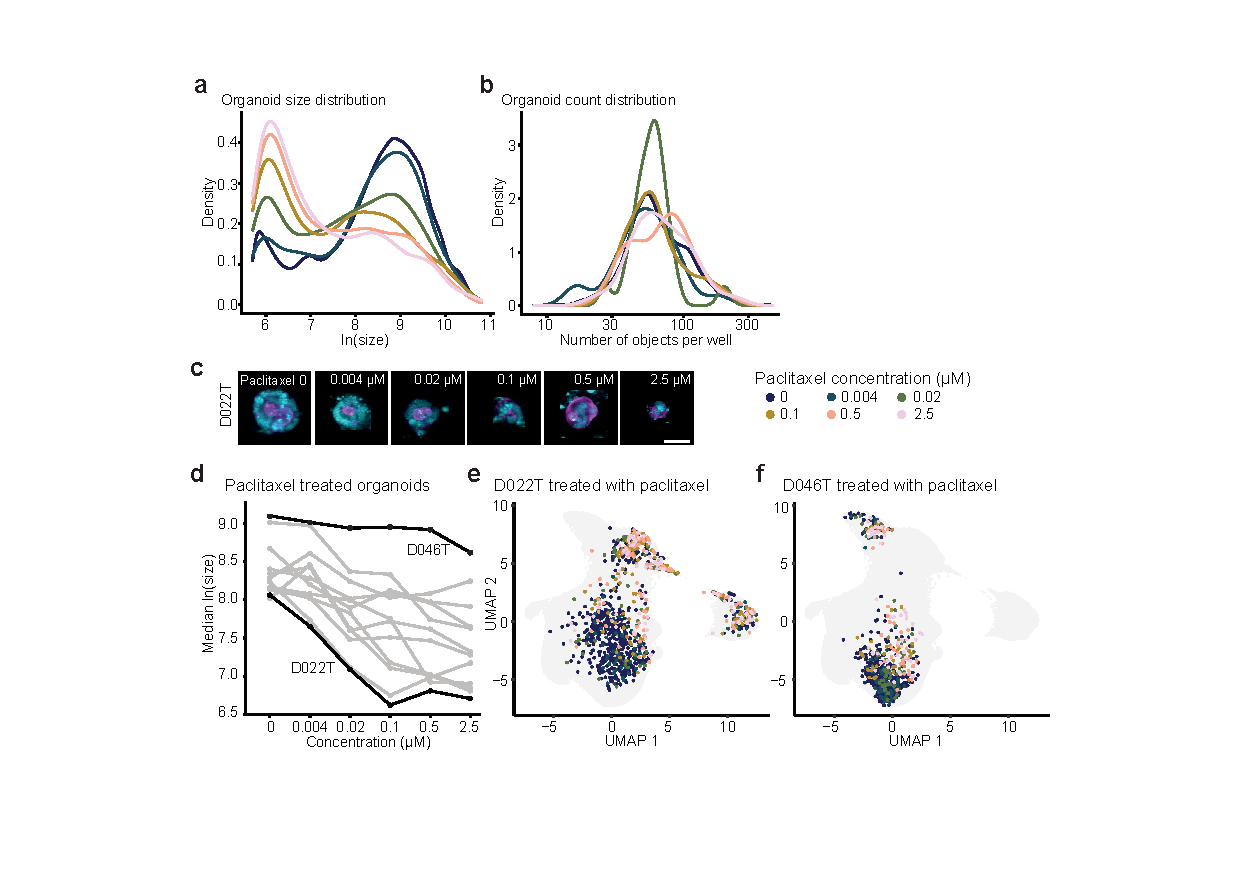
\includegraphics[width=\textwidth,
                height=\textheight,
                keepaspectratio]{figures/promise/pdf/fig_2_2.pdf}
\caption[Organoid phenotype-profiles capture treatment specific changes in organoid viability]{\textbf{Organoid phenotype-profiles capture treatment specific changes in organoid viability. a} Distribution of organoid size at different concentrations of Paclitaxel. Shown is a random sample of 30\% of all Paclitaxel treated organoids for this and following figures. \textbf{b} Distribution of organoid number per well at different concentrations of Paclitaxel. \textbf{c} Example images of D022T organoids treated with Paclitaxel. \textbf{d} Dose-response relationship of organoid size and paclitaxel dose. D022T and D046T are highlighted. \textbf{e} UMAP of organoid morphology highlighting D022T organoids treated at different concentrations of Paclitaxel. \textbf{f} UMAP of organoid morphology highlighting D046T organoids treated at different concentrations of Paclitaxel. Figure adapted from \textit{The drug-induced phenotypic landscape of colorectal cancer organoids} \citep{Betge2022-kr}}
\label{fig_222}
\end{figure}
\bigbreak

To test whether a more accurate prediction of organoid viability was achievable by using all available imaging data, I used a previously trained set of random forest classifiers (live/dead classifiers, LDC). These classifiers were trained on individual organoid phenotype profiles to distinguish between negative and positive control treatments (DMSO, Bortezomib and SN-38). 

\bigbreak
When applying the classifier to the whole imaging dataset and visualizing predictions via UMAP, organoids within previously identified small-object regions 2, 3 and 4 had the highest probabilities for death (Figure \ref{fig_222} b). 

\bigbreak
Not only organoid size, but also the viability classified (LDC) correlated with luminescence-based viability (CTG) measurements (Figure \ref{fig_222} b and c). In fact, the trained classified, together with organoid size showed the most robust correlation with luminescence-based viability measurements across all profiled organoid lines (Figure \ref{fig_222} d), while other simple features, such as DAPI, Actin, and permeability (DeadGreen) intensity were less suitable to predict the viability of organoids. 

\bigbreak
In conclusion, organoid size is an informative metric to approximate organoid viability, but is biased by line-specific differences in organoid size. Models consuming more comprehensive morphological information can achieve even higher predictive performance of organoid viability. 

\clearpage
\begin{figure}[h]
\centering
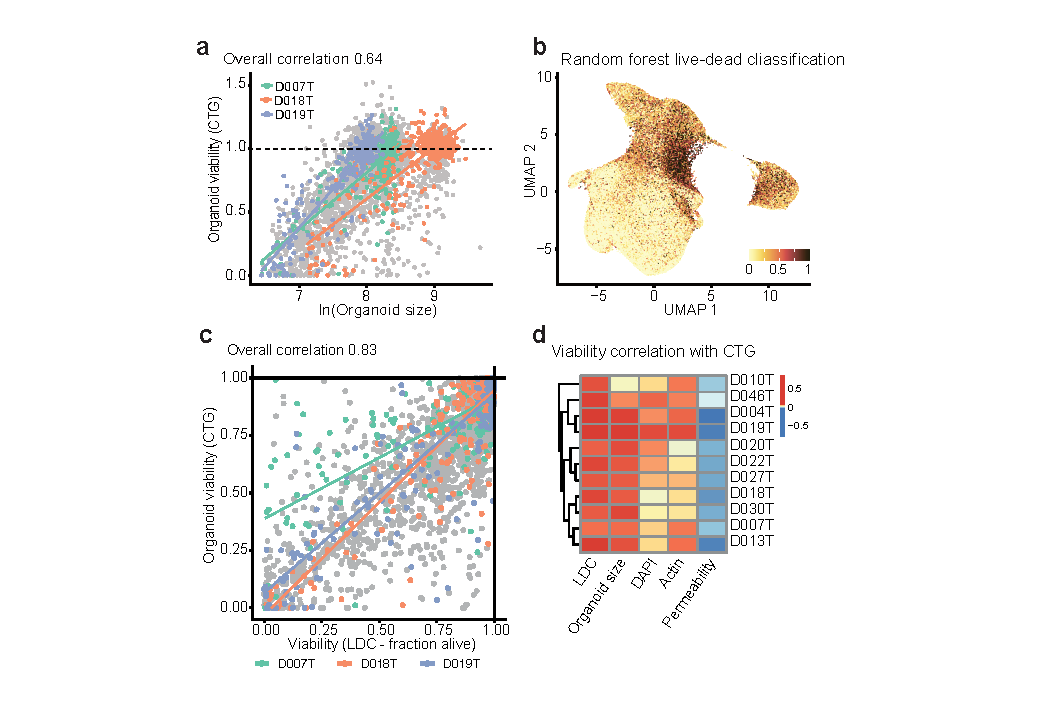
\includegraphics[width=\textwidth,
                height=\textheight,
                keepaspectratio]{figures/promise/pdf/fig_2_3.pdf}
\caption[Organoid phenotype-profiles reflect ATP-dependent viability measurements]{\textbf{Organoid phenotype-profiles reflect ATP-dependent viability measurements. a} Association of organoid size of selected example lines with organoid viability determined by luminescence-based, ATP-dependent viability profiling with CellTiter-Glo (CTG), which was performed in parallel with imaging on a subset of drug treatments. \textbf{b} UMAP visualization of dead organoids within our dataset, based on supervised machine learning of organoid viability using classifiers trained on positive- (high-dose bortezomib and SN-38) and negative (DMSO) controls (live-dead classifiers, LDC). \textbf{c} Association of organoid size of selected example lines with organoid viability determined by luminescence-based, ATP-dependent viability profiling with CellTiter-Glo (CTG), which was performed in parallel with imaging on a subset of drug treatments for benchmarking. \textbf{d} UMAP visualization of dead organoids within our dataset, based on supervised machine learning of organoid viability using classifiers trained on positive- (high-dose Bortezomib and SN-38) and negative (DMSO) controls (live-dead classifiers, LDC). \textbf{e} Association of LDC and example organoid features (size, DAPI, actin and permeability dye intensities) with benchmark CTG viability read out. Figure created with support from Jan Sauer (LDC classifier training) and adapted from \textit{The drug-induced phenotypic landscape of colorectal cancer organoids} \citep{Betge2022-kr}}
\label{fig_223}
\end{figure}
\bigbreak

\subsection{Drug induced organoid phenotypes correspond to drug mechanism of action}

An advantage of image-based profiling over one dimensional cell viability measurements in drug discovery is the ability to use the high dimensional drug-induced phenotype-profiles to identify active but not necessarily lethal small molecules and estimate their mechanism of action through clustering with other well-annotated small molecules. 

\bigbreak
To test whether this approach could be used in cancer organoids, I used a weakly supervised learning approach to identify treatment effect vectors and group them by similarity. With the support of Jan Sauer, logistic regression models to separate individual compound-treated organoids from unperturbed controls were trained. The resulting normal vector between control- and treated organoid profiles was referred to as the treatment effect vector. Next, every model’s ability to separate treated and untreated organoids was scored (AUROC, mean from bootstrapped modeling with values ranging from 0.5 to 1) to identify active treatments that induce a robust change in organoid morphology (Figure \ref{fig_230} a, b). I referred to the AUROC as the drug activity score. An AUROC of 1 is associated with a strong difference in organoid morphology, while an AUROC of 0.5 corresponds to no identifyable difference. Drug activity (as expressed by an activity score larger than an arbitrary cutoff of 0.85) was necessary but not sufficient for a viability effect (Figure \ref{fig_230} c). A fraction of drugs led to identifiable changes in organoid morphology but were not classified as lethal by the LDC model. To test whether active drugs systematically lead to organoid phenotypes that are informative of mechanism of action, the cosine distance between concatenated treatment effect vectors was determined. This approach led to a clustering of specific mode-of-actions, including inhibitors of MEK, Aurora kinase, CDK, mTOR, AKT, EGFR or GSK3 (Figure \ref{fig_231} a). 

\begin{figure}[h]
\centering
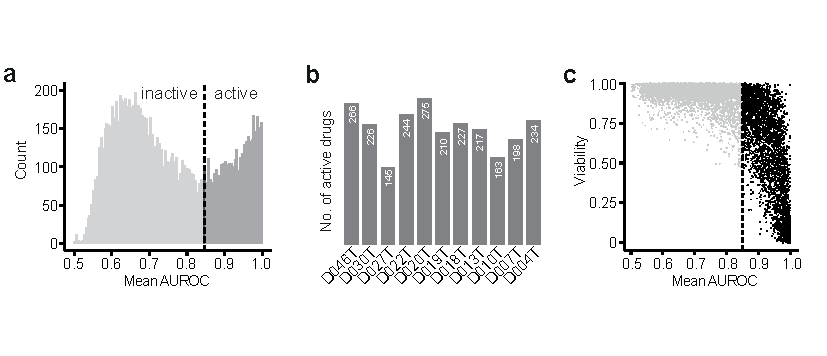
\includegraphics[width=\textwidth,
                height=\textheight,
                keepaspectratio]{figures/promise/pdf/fig_3_0.pdf}
\caption[Distribution of drug activity scores]{\textbf{Distribution of drug activity scores. a} Distribution of AUROC scores across all studied organoid models and treatments. \textbf{b} Number of active treatments per organoid line. \textbf{c} Relationship of drug activity and predicted organoid viability. Figure created with support from Jan Sauer (drug activity classifier training, LDC classifier training) and adapted from \textit{The drug-induced phenotypic landscape of colorectal cancer organoids} \citep{Betge2022-kr}}
\label{fig_230}
\end{figure}
\bigbreak


\bigbreak
I next validated the previous approach, and tested alternative methods to 1) quantify treatment activity and 2) cluster treatment effects by similarity. The AUROC score which was previously used to define active treatments, correlated with the euclidean distance of phenotype profiles (Figure \ref{fig_232} a) and showed moderate variance when evaluated for stability by bootstrapping (Figure \ref{fig_232} b). Similarly, evaluating an alternative clustering method based on phenotype profile averaging (instead of concatenating) followed by Pearson correlation (instead of cosine distance determination) led to an overall similar clustering result of treatments (Figure \ref{fig_232} c). 

\begin{figure}[h!]
\centering
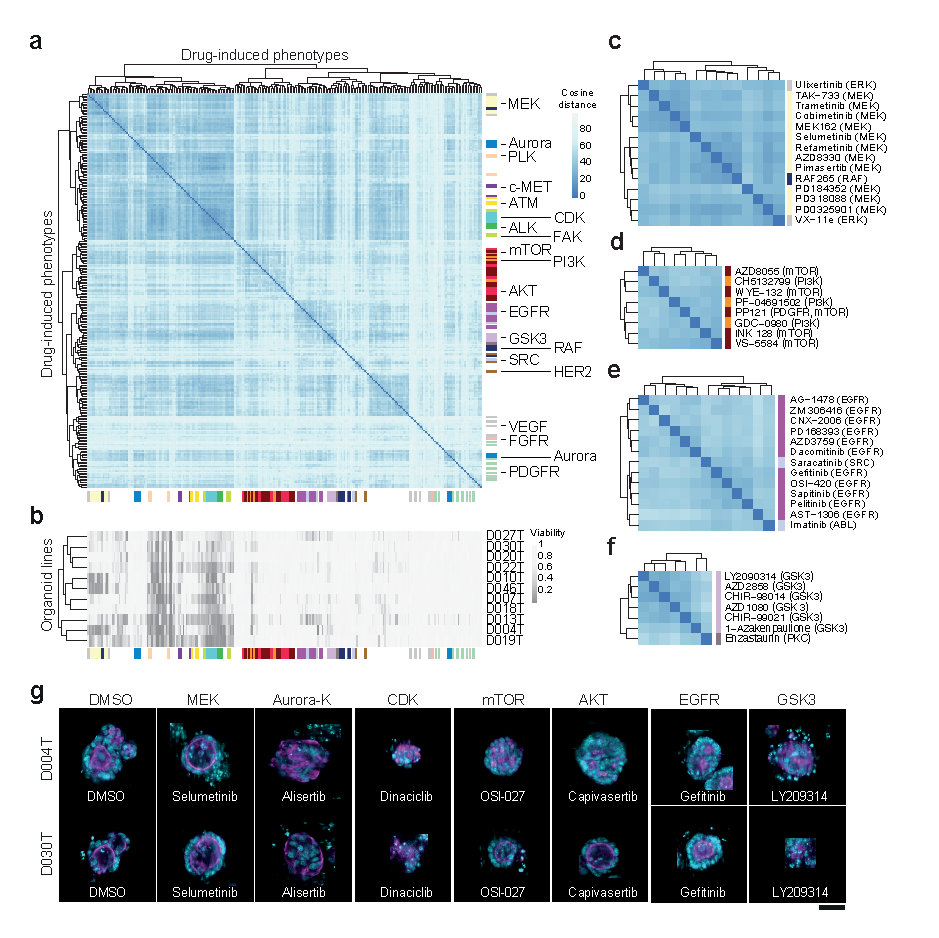
\includegraphics[width=\textwidth,
                height=\textheight,
                keepaspectratio]{figures/promise/pdf/fig_3_1.pdf}
\caption[Clustering of treatment effects captures mechanism of action]{\textbf{Clustering of treatment effects captures mechanism of action. a} Hierarchical clustering of treatment effect vectors across all observed organoid models. Clustering is based on the cosine distance of concatenated treatment effect vectors. Sidebars are color-coded by the primary annotated target. \textbf{b} Viability classifier predictions (LDC classifier) for organoids, arranged according to the clustering in panel a. \textbf{c-f} Magnified regions from panel a showing clusters of small molecule inhibitors targeting MEK, mTOR, EGFR, and GSK3. \textbf{g} Representative images of treatment-induced organoid phenotypes for seven clusters of small molecules (cyan = DNA, magenta = actin, yellow = cell permeability; average images were selected and embedded in black background; scale bar: 50µm). Figure created with support from Jan Sauer (drug activity classifier training, LDC classifier training) as well as Johannes Betge (example picture selection) and adapted from \textit{The drug-induced phenotypic landscape of colorectal cancer organoids} \citep{Betge2022-kr}.}
\label{fig_231}
\end{figure}
\bigbreak

Compounds with related, but not identical, targets also induced related phenotypes, for example MEK inhibitors clustered with specific RAF- and ERK inhibitors (Figure \ref{fig_231} c-f) or AKT and PI3K inhibitors were part of a cluster mainly containing mTOR targeting compounds. The clustering also suggested additional mode-of-actions or off-target effects for well-described compounds. For example, the PKC inhibitor Enzastaurin was associated with GSK3 inhibitors, substantiating a previously described interaction with the alpha and beta subunits of GSK3 \citep{Kotliarova2008-tz, Klaeger2017-vu} (Figure \ref{fig_231} f). 

\bigbreak
To assess whether morphological profiles of active drug treatments were primarily driven by differences in organoid viability, LDC classifier predictions were aligned with the phenotypic clustering (Figure \ref{fig_231} b). While a large cluster of lethal treatments (including molecules targeting ATM, JAK, PLK, CDK) existed, the majority of clusters were caused by non-lethal phenotypes - including those induced by inhibitors of AKT, mTOR, EGFR or GSK3.

\bigbreak

Manual inspection of several phenotypes (Figure \ref{fig_231} g) revealed recurring characteristic treatment-target dependent phenotypes. Most notably, MEK inhibitors led to reorganization towards more cystic organoid architecture. These target dependent phenotypes were observable across organoid lines and drugs.


\begin{figure}[h!]
\centering
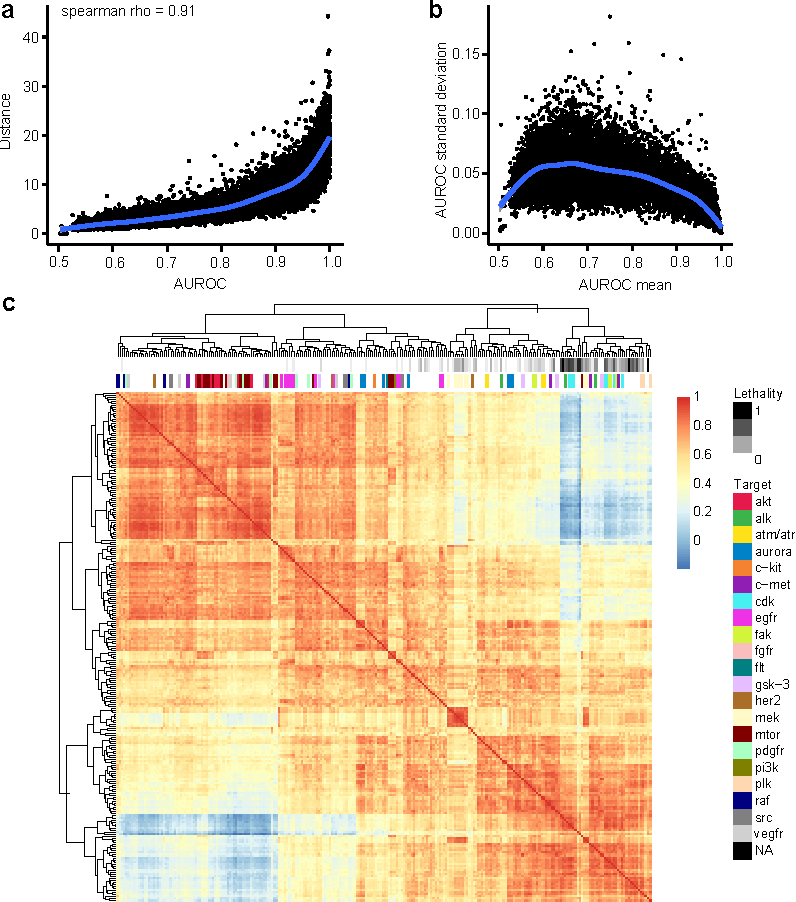
\includegraphics[width=\textwidth,
                height=\textheight,
                keepaspectratio]{figures/promise/pdf/fig_3_2.pdf}
\caption[Validation of treatment activity and effect quantification]{\textbf{Validation of treatment activity and effect quantification. a} Relationship between eucledian distance of treatment effect vectors and classifier AUROC. The spearman correlation between the two metrics is shown in the top left. Smoothed line represents a loess fit. \textbf{b} Relationship between standard deviation of the AUROC score across bootstrapping runs for one treatment and the mean AUROC score of the treatment. Smoothed line represents a loess fit. \textbf{c} Hierarchical clustering of treatment effect vectors across all observed organoid models. Clustering is based on the eucledian distance of average treatment effect vectors. Sidebars are color-coded by the primary annotated target.}
\label{fig_232}
\end{figure}
\bigbreak


\newpage

\section{Multi-omics factor analysis identifies shared factors linking morphology, genomic data and drug activity}

A limitation of image-based profiling experiments is that both unperturbed and drug induced phenotypes are challenging to interpret in terms of their underlying biology. I hypothesized that, in the presence of multiple in vitro models with both phenotype and transcriptome measurements, links between the two data modalities can be learned. 

\begin{figure}[h!]
\centering
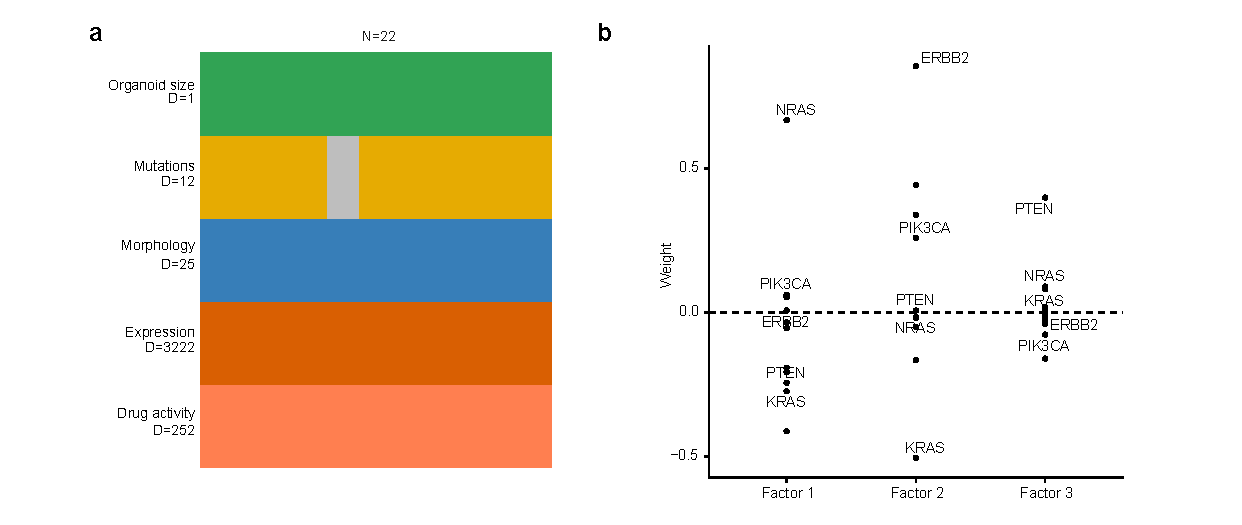
\includegraphics[width=200,
                height=\textheight,
                keepaspectratio]{figures/promise/pdf/fig_4_2.pdf}
\caption[Overview of input data for MOFA modeling]{\textbf{Overview of input data for MOFA modeling. a} 22 observations of 11 models across 5 different views (size, mutation, morphology, gene expression and treatment activity) were integrated in the model. Missing data is shown in grey. "D" represents the vector length of the respective view. Figure adapted from \textit{The drug-induced phenotypic landscape of colorectal cancer organoids} \citep{Betge2022-kr}.}
\label{fig_242}
\end{figure}

\bigbreak
To learn a multi-view representation of unperturbed organoid morphology, unperturbed organoid size, gene expression, somatic mutations, and drug activity, multi-omics factor analysis (MOFA) was performed on the support set data. MOFA is a matrix factorization method built upon group factor analysis, with decomposes a set of different measurements into a shared table of factors scoring each observed sample and a set of corresponding tables linking each factor to features in the set of original measurements \citep{Argelaguet2018-yi}. 

\bigbreak
The support data used to fit the MOFA model consisted of a set of five matrices, each with 22 observations (rows) representing 11 organoid models with 2 replicates per model (Figure \ref{fig_241} a). Each matrix represented a data modality/view (mutation, morphology, gene expression, etc.) and had a range of attributes (columns). When trained with a low number of k = 3 factors, MOFA recovered factors explaining ca. 41-24\% of variance across the different data modalities, with the first two factors accounting for ca. 29-17\% in aggregate (Figure \ref{fig_240} a). While gene expression, mutations and drug activity profiles for organoid lines contributed to all factors, factor 1 captured an exceptional amount of variation in median organoid size (ca. 39\%). In contrast, factor 2 was primarily capturing variation within baseline organoid morphology (ca. 16\%) (Figure \ref{fig_240} a).

\begin{figure}[h!]
\centering
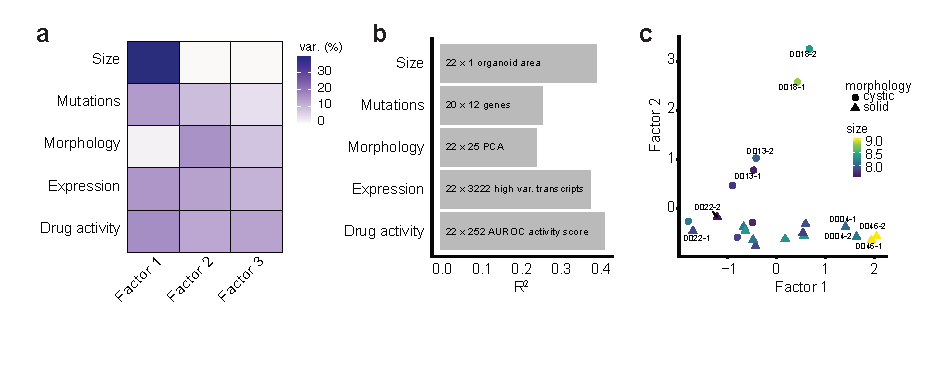
\includegraphics[width=\textwidth,
                height=\textheight,
                keepaspectratio]{figures/promise/pdf/fig_4_0.pdf}
\caption[Mulit-omics factor analysis of organoid profiles]{\textbf{Mulit-omics factor analysis of organoid profiles. a-b} Variance decomposition of the MOFA model. Shown is the variance explained for every factor and data modality, as well as only by modality. \textbf{c} Factor scores for individual observations. The shapes represent the manually determined morphology label and color average organoid size. Figure adapted from \textit{The drug-induced phenotypic landscape of colorectal cancer organoids} \citep{Betge2022-kr}.}
\label{fig_240}
\end{figure}

\bigbreak
Overall, MOFA factors explained up to 40\% of variance in median organoid size, drug activity and gene expression, while less than 30\% of variance in baseline organoid morphology was explained by the model (Figure \ref{fig_240} b). Organoid lines D046T and D004T stood out as lines with the strongest score for factor 1, while lines D018T and D013T had the strongest score in factor 2. Visual inspection of organoids revealed that organoid lines with a higher factor 1 score tended to be larger in size and organoids with high factor 2 score tended to have a more cystic organoid architecture based on manual classification (Figure \ref{fig_240} c). No interpretable morphological differences between factor 3 low and high organoids were identifiable, so the subsequent analysis was focused on the first two interpretable factors generated by MOFA. To ensure that the learnt embeddings, especially with regards to size and morphology differences, were not biased by the dimensionality of individual views within the support set, I explored the gene expression data directly and plotted organoid models by their manual morpholoical classiciation (Figure \ref{fig_241} a) and measured size (Figure \ref{fig_241} b). Principal component analysis of high variance probes recovered the same observations. To summarize, unsupervised multi-view representation learning with MOFA identified factors within the dataset that explained variation between organoid lines across different data modalities, including organoid morphology and median organoid size. 

\begin{figure}[h!]
\centering
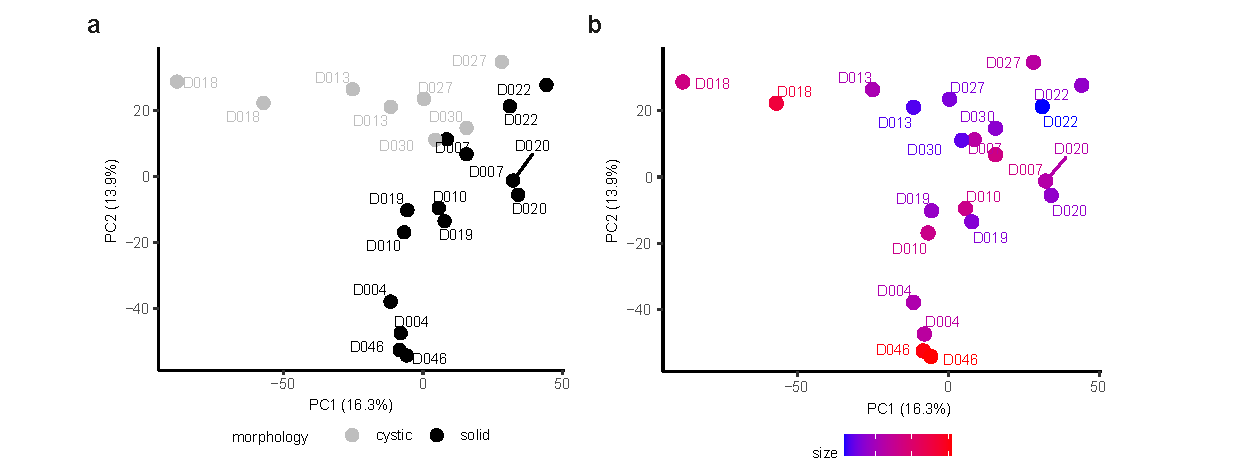
\includegraphics[width=\textwidth,
                height=\textheight,
                keepaspectratio]{figures/promise/pdf/fig_4_1.pdf}
\caption[Validation of characteristic organoid phenotypes by expression analysis]{\textbf{Validation of characteristic organoid phenotypes by expression analysis. a} PCA of gene expression data for organoid models. Observations are color-coded by the manually determined morphology label. \textbf{b} Identical PCA of expression data, color-coded by average organoid size.}
\label{fig_241}
\end{figure}


\newpage
\subsection{An IGF1R signaling program is associated with increased organoid size, EGFR inhibitor resistance and can be induced by mTOR inhibition}

Differences in organoid size are a contributing factor to intra- and inter-organoid line heterogeneity. Organoid size was influenced by both organoid line and drug treatments and was associated with factor 1 scores (Figure \ref{fig_261} a). An unsupervised gene set enrichment analysis (GSEA) for Reactome pathways across factor 1 loadings showed an enrichment for IGF1R signaling and mitogen-activated protein kinase signaling related genes (Figure \ref{fig_261} b). 

\begin{figure}[h!]
\centering
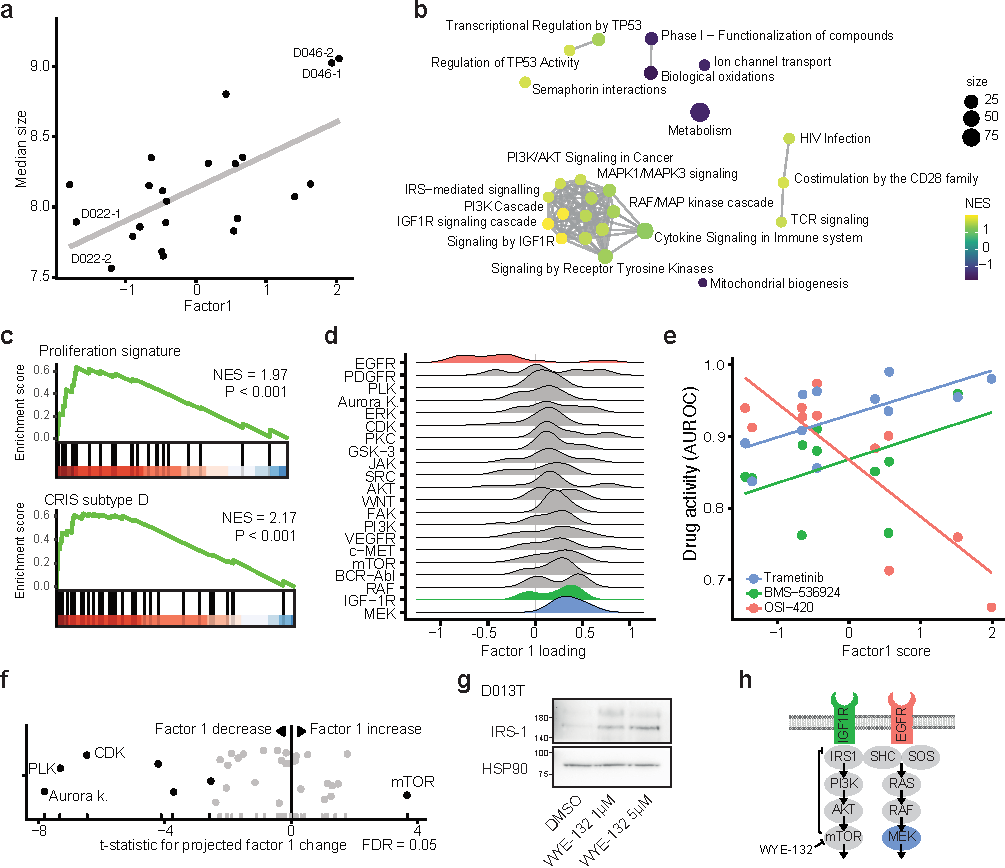
\includegraphics[width=\textwidth,
                height=\textheight,
                keepaspectratio]{figures/promise/pdf/fig_6_1.pdf}
\caption[Factor 1 overview]{\textbf{Factor 1 overview. a} Association between organoid size and factor 1 score. \textbf{b} GSEA network of factor 1 gene expression loadings. An edge connects Reactome pathways with more than 20\% overlap. \textbf{c} GSEA of the proliferation signature and the colorectal cancer CRIS-D subtype over ranked factor 1 gene expression loadings (ranking from high factor 1 to low factor 1 loading). \textbf{d} Distributions of treatment activity score loadings grouped by targets for factor 1. \textbf{e} Relationship of selected treatment activity scores (AUROC) with factor 1 score. \textbf{f} Projection of factor 1 scores for drug-induced phenotypes. Highlighted are drug targets leading to a significant change in projected factor scores across all organoid lines (ANOVA). \textbf{g} Western blot of IRS-1 protein abundance under mTOR inhibition for a representative organoid line (D013T). \textbf{h} Illustration of IGF1R signaling pathway with highlighted drug targets. Shown is the disinhibition of mTOR mediated IRS-1 repression after treatment with mTOR inhibitors. Figure adapted from \textit{The drug-induced phenotypic landscape of colorectal cancer organoids} \citep{Betge2022-kr}.}
\label{fig_261}
\end{figure}
\bigbreak

In fact, the IGF signaling related transcripts H19 (rank 1) and IGF2 (rank 13) were among the strongest contributors to factor 1. This increase in proliferative signaling was confirmed by GSEA of a previously identified intestinal proliferation signature by Merlos-Suarez et al. \citep{Merlos-Suarez2011-gd} (Figure \ref{fig_261} c). 

\bigbreak
To better understand clinical correlates to the identified gene expression patterns, I tested for nerichment of molecular subtype profiles stemming from an analysis of cancer-cell intrinsic transcription \citep{Isella2017-bm}. Factor 1 showed an enrichment for CRIS D, a molecular subtype linked to IGF2 overexpressing tumors, loss of IGF2 imprinting and resistance to EGFR inhibitor therapy (Figure \ref{fig_261} c). Conversely, I observed a depletion for CRIS C, which has been linked to EGFR dependency (Figure \ref{fig_262} a and b). In fact, activity of EGFR inhibitors was the strongest contributor to a negative factor 1 score while IGF1R and MEK inhibitor activity contributed to a positive factor 1 score (Figure \ref{fig_261} d-e and Figure \ref{fig_262} c-e).

\begin{figure}[h!]
\centering
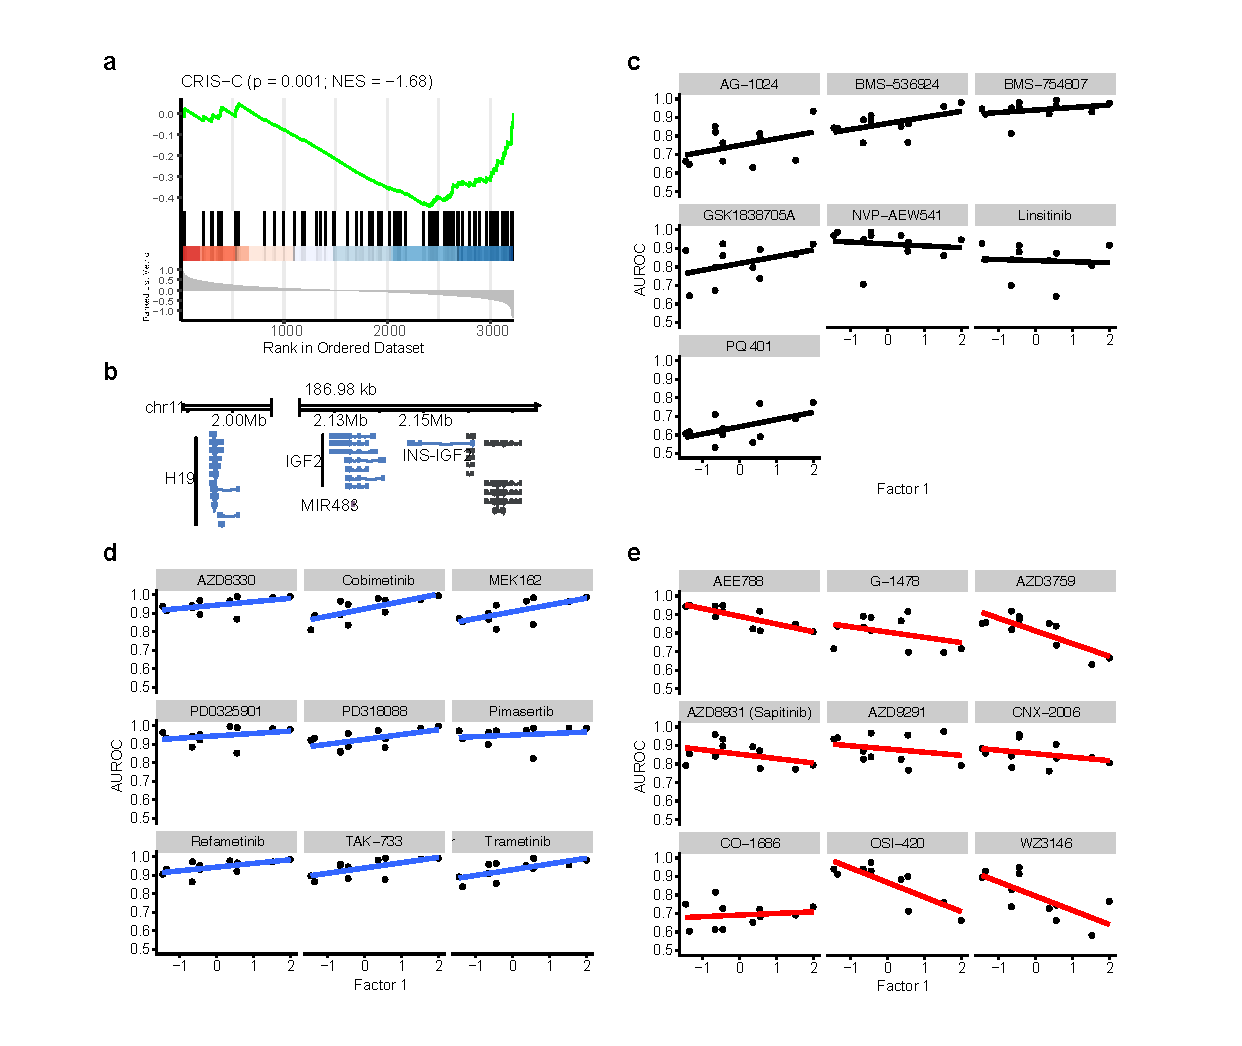
\includegraphics[width=\textwidth,
                height=\textheight,
                keepaspectratio]{figures/promise/pdf/fig_6_2.pdf}
\caption[Factor 1 extended overview]{\textbf{Factor 1 extended overview. a} GSEA of the CRIS C subtype signature over ranked factor 1 gene expression loadings. \textbf{b} IGF2 and H19 locus in the human genome. \textbf{c-e} Association between treatment activity scores and factor 1 scores for three classes of compounds, targeting IGF1R, MEK and EGFR, respectively. Figure adapted from \textit{The drug-induced phenotypic landscape of colorectal cancer organoids} \citep{Betge2022-kr}.}
\label{fig_262}
\end{figure}

\bigbreak
Once a representation space has been learnt through the support set, a core component of image based profiling is to estimate the effect of observed treatments on identified factors. To test whether small molecule treatments shifted organoids in factor space, the morphological features of treated organoids in the query set were projected into factor space. This projection was done based on generating the pseudoinverse of the loading matrix and multiplying with the average phenotypic profiles of treated organoids. While only morphological data was available during for observations in the query set, this inversion enabled interpreting treatment-induced phenotypes in a representation space previously learnt from multi-view data of unperturbed organoids in the support set. 

\bigbreak
A group of cell cycle related kinase inhibitors targeting polo like kinases, Aurora kinases and cyclin dependent kinases shifted organoids to a low factor 1 score (Figure \ref{fig_261} f). In contrast, mTOR inhibitor treatment increased factor 1 scores in cancer organoids (Figure \ref{fig_261} f). Given the observation that factor 1 was associated with IGF-1R signaling and mTOR inhibitor treatment led to an increase in factor 1 scores, I hypothesized that mTOR inhibition leads to a reactive upregulation of IGF1R signaling in cancer organoids. In fact, inhibition of mTOR signaling had previously been linked to transcriptional disinhibition of IRS-1 in a negative feedback loop \citep{OReilly2006-fc} and  reactive induction of IGF1R signaling had previously been described as a resistance mechanism to small molecule mTOR inhibitors in cancer \citep{Sharma2010-qa}. When testing this hypothesis in patient derived organoids, a dose-dependent increase of IRS-1 protein abundance in organoids treated with the ATP competitive mTOR inhibitor WYE-132 was observable (Figure \ref{fig_261} g and h). 

\bigbreak
To summarize, factor 1 described an organoid state with relatively large organoid size, elevated IGF1R dependent mitogenic signaling which could be induced by inhibiting an mTOR dependent negative feedback loop in patient derived cancer organoids.

\newpage
\subsection{An LGR5+ program is associated with cystic organoid architecture, Wnt signaling inhibitor sensitivity, and can be induced by inhibition of MEK}

Besides size differences, a particularly strong recurring organoid phenotype was the presence of a cystic organoid architecture, seen for example in untreated D018T organoids and organoids treated with MEK inhibitors (Figure \ref{fig_140} and \ref{fig_231}). In the cystic state, which was observed in factor 2 high organoid lines, organoids consisted of a monolayer of uniform cells lining a central spherical lumen with a distinct apico-basally oriented actin cytoskeleton (Figure \ref{fig_251} a and b). This phenotype was reminiscent of organoid morphologies previously seen in APC-/- or Wnt ligand treated human intestinal organoids \citep{Matano2015-zw}. 

\begin{figure}[h!]
\centering
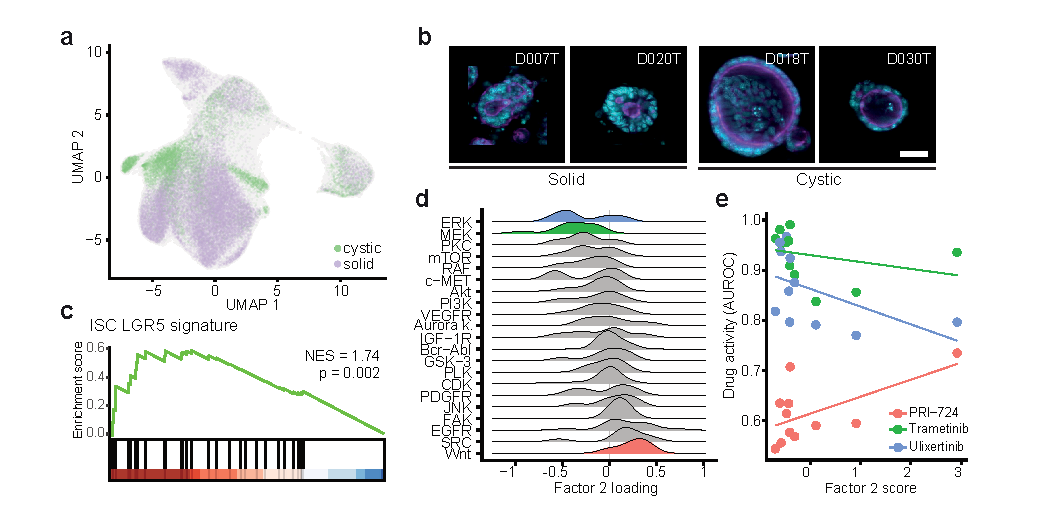
\includegraphics[width=\textwidth,
                height=\textheight,
                keepaspectratio]{figures/promise/pdf/fig_5_1.pdf}
\caption[Factor 2 overview]{\textbf{Factor 2 overview. a} UMAP of observed organoids. Color labels represent the manually determined morphology labels. \textbf{b} Representative images of solid and cystic organoid phenotypes (cyan = DNA, magenta = actin, yellow = cell permeability; average images were selected and embedded in black background; scale bar: 50µm). \textbf{c} GSEA of LGR5 gene expression signature over ranked factor 2 gene expression loadings (ranking from high factor 2 to low factor 2 loading). \textbf{d} Distributions of treatment activity score loadings grouped by targets for factor 2. \textbf{e} Relationship of selected treatment activity scores (AUROC) with factor 2 score. Example images curated with support from Johannes Betge. Figure adapted from \textit{The drug-induced phenotypic landscape of colorectal cancer organoids} \citep{Betge2022-kr}.}
\label{fig_251}
\end{figure}
\bigbreak

To test if factor 2 comprised Wnt signaling and intestinal stem cell identity related gene expression programs, gene set enrichment analyses (GSEA) was performed for cell identity signatures previously described by Merlos-Suarez et al. \citep{Merlos-Suarez2011-gd}. GSEA revealed an enrichment of Lgr5+ stem cell signature-related genes for the factor 2 loadings (FDR=0.002, NES=1.74) (Figure \ref{fig_251} c). Activity of Wnt signaling inhibitors and EGFR inhibitors were the strongest average contributors to a positive factor 2 score (t statistic = 3.02, FDR = 0.046 and t statistic = 3.08, FDR = 0.046, respectively), while activity of ERK and MEK inhibitors were associated with a low factor 2 score (Figure \ref{fig_251} d), albeit not significantly. As expected from these results, factor 2 high organoid lines showed a stronger morphological response to the Wnt pathway inhibitor PRI-724. (Figure \ref{fig_251} e).

\begin{figure}[h!]
\centering
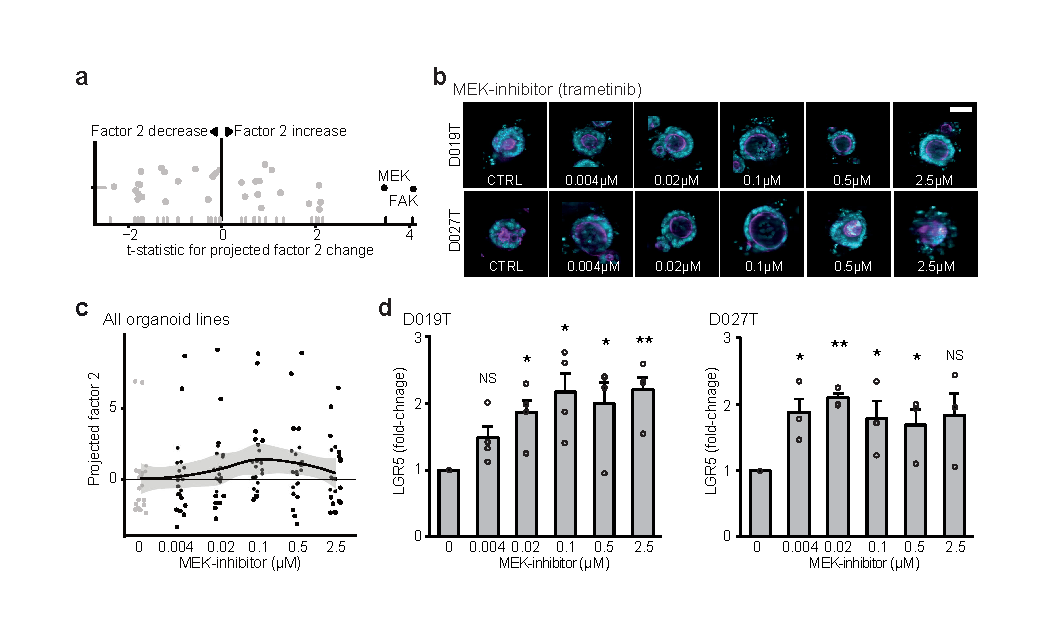
\includegraphics[width=\textwidth,
                height=\textheight,
                keepaspectratio]{figures/promise/pdf/fig_5_3.pdf}
\caption[Factor 2 extended overview]{\textbf{Factor 2 extended overview. a} Projection of factor 2 scores for drug-induced phenotypes. Highlighted are drug targets leading to a significant change in projected factor scores across all organoid lines (ANOVA). \textbf{b} Representative images of organoid phenotypes across 5 increasing concentrations of MEK inhibitor treatment and negative control (0.1\% DMSO) (cyan = DNA, magenta = actin, yellow = cell permeability; average images were selected and embedded in black background; scale bar: 50µm). \textbf{c} Projected dose-dependent changes in factor 2 scores after treatment with the MEK inhibitor Binimetinib. The horizontal black line indicates median factor 2 values of all binimetinib treatment observations. A loess fit with 95\% confidence interval (grey background) is provided. \textbf{d} Dose-dependent changes in LGR5 transcript abundance after treatment with the MEK inhibitor trametinib, as assessed by qPCR, data from 3 (D027T) and 4 (D019T) independent replicates are presented as mean + s.e.m. *p < 0.05, **p < 0.005, NS = not significant, two-sided Student’s t test. p values: D019T: p = 0.061 (0.004 µM), p = 0.0196, (0.02 µM), p = 0.0187 (0.1 µM), p = 0.024 (0.5 µM), P = 0.0024 (2.5 µM), D027T: p = 0.0051 (0.004 µM), p = 0.00038, (0.02 µM), p = 0.045 (0.1 µM), p = 0.048 (0.5 µM), P = 0.090 (2.5 µM). Example images curated with support from Johannes Betge. Figure adapted from \textit{The drug-induced phenotypic landscape of colorectal cancer organoids} \citep{Betge2022-kr}.}
\label{fig_253}
\end{figure}
\bigbreak

Next, I again projected phenotype profiles of treated organoids and approximated how drug treatment shifted organoids along factor 2. I observed MEK and focal adhesion kinase inhibitors significantly shifting all tested organoid lines towards higher factor 2 scores (Figure \ref{fig_253} a). This change in factor 2 scores was concentration dependent for MEK inhibitors and coincided with a visual shift in organoid morphology (Figure \ref{fig_253} b and c). Given the observation that factor 2 was enriched for an LGR5+ stem cell signature, the expression of LGR5 transcripts at different concentrations of MEK inhibitor treatment was measured and an analogous dose-dependent increases in transcript abundance was observed (Figure \ref{fig_253} d). These findings were in agreement with the observation that MEK inhibitor activity had a negative contribution to factor 2 \ref{fig_251} d) - While organoids are shifted to a factor 2 high state by MEK inhibition, within the factor 2 high state itself, organoids are relatively insensitive to this treatment. In summary, factor 2 represents an organoid state with cystic architecture, increased expression of LGR5+ stem cell related genes and increased sensitivity to Wnt signaling inhibitors that could be induced by MEK inhibition.

\end{flushleft}

